\chapter{Proofs}

\compcover*\label{lem:compcover2}
\begin{flushright}\hyperref[lem:compcover]{\upsym}\end{flushright}
\begin{proof}
	For $x \in C$ let $\delta_x > 0$ be such that $B_{\delta_x}(x) \subset \Omega.$ (Which exists because $\Omega$ is open.)\\
	Then, $C \subset \displaystyle\bigcup_{x \in C}B_{\delta_x/2}(x).$\\
	Since $C$ is compact, only finitely many of $B_{\delta_x/2}(x)$ cover $C.$ Let $I = \{x_1, \ldots, x_n\}$ be such that $C \subset \displaystyle\bigcup_{x \in I}B_{\delta_x/2}(x).$

	Define $D =\displaystyle\bigcup_{x \in I}\overline{B_{\delta_x/2}(x) }.$

	Clearly, $C \subset  \displaystyle\bigcup_{x \in I}B_{\delta_x/2}(x) \subset \operatorname{int} D.$

	Moreover, $D$ is union of finitely many closed balls and hence, is closed and bounded and thus, compact.

	Lastly, $D = \displaystyle\bigcup_{x \in I}\overline{B_{\delta_x/2}(x)} \subset \displaystyle\bigcup_{x \in I}B_{\delta_x}(x) \subset \Omega,$ completing the proof.
\end{proof}

\amgmhm*\label{thm:amgmhm2}
\begin{flushright}\hyperref[thm:amgmhm]{\upsym}\end{flushright}
\begin{proof} 
	Note that it is enough to prove $\text{AM} \ge \text{GM}$ since the other inequality will follow by considering the reciprocals.\\
	We prove $\text{AM} \ge \text{GM}$ via induction. The case $n = 2$ (and $n=1$) is trivial and follows from manipulating $(\sqrt{a_1} - \sqrt{a_2})^2 \ge 0.$\\
	Assume that it is true for $n.$ We prove it for $n + 1.$\\
	Let $A_k \vcentcolon= \dfrac{1}{k}(a_1 + \cdots + a_k)$ and $G_k \vcentcolon= (a_1\cdots a_k)^{1/k}.$\\
	Then, we have
	\begin{align*} 
		A_{n+1} &= \dfrac{1}{n+1}(a_1 + \cdots + a_{n+1})\\
		&= \dfrac{1}{n+1}(nA_n + a_{n+1})\\
		&\ge \dfrac{1}{n+1}(nG_n + a_{n+1})\\
		&= \dfrac{1}{n+1}\left(nG_{n+1}\left(\dfrac{G_{n+1}}{a_{n+1}}\right)^{1/n} + a_{n+1}\right) & (G_{n+1}^{n+1} = G_n^na_{n+1})\\
		&= G_{n+1}\cdot\dfrac{1}{n+1}\left(n\left(\dfrac{G_{n+1}}{a_{n+1}}\right)^{1/n} + \dfrac{a_{n+1}}{G_{n+1}}\right)\\
		\implies \dfrac{A_{n+1}}{G_{n+1}} &\ge\dfrac{1}{n+1}\underbrace{\left(n\left(\dfrac{G_{n+1}}{a_{n+1}}\right)^{1/n} + \dfrac{a_{n+1}}{G_{n+1}}\right)}_{(*)}
	\end{align*}
	If we prove that $(*) \ge n+1,$ then we are done.\\
	Call $\dfrac{G_{n+1}}{a_{n+1}} =\vcentcolon \theta^{-n}.$\\
	Thus, we want to show that $n\theta^{-1} + \theta^n \ge n+1.$\\
	Note the following equivalences
	\begin{align*} 
		n\theta^{-1} + \theta^n \ge n+1 &\iff \theta^{n+1} - \theta n - \theta + n \ge 0\\
		&\iff \theta(\theta^n - 1) - n(\theta - 1) \ge 0\\
		&\iff \theta(\theta - 1)(\theta^{n-1} + \cdots + 1) - n(\theta - 1) \ge 0\\
		&\iff (\theta - 1)[\theta^n + \cdots + \theta - n] \ge 0\\
		&\iff (\theta - 1)[(\theta^n - 1) + \cdots + (\theta - 1)] \ge 0.
	\end{align*}
	The last inequality holds for $\theta = 1,$ $\theta > 1,$ and $0 < \theta < 1.$ Thus, we are done!
\end{proof}

\coramgmhm*\label{cor:coramgmhm2}
\begin{flushright}\hyperref[cor:coramgmhm]{\upsym}\end{flushright}
\begin{proof}
	\begin{enumerate}[label = (\roman*)]
		\item Clearly true for $a = 1.$ We assume $a > 1.$ Proving this case is sufficient. (Why?)\\
		For $n \ge 2,$ apply AM-GM to $\underbrace{1, \ldots, 1,}_{n-1} a$ to get
		\begin{equation*} 
			1 \le \sqrt[n]{a} \le \dfrac{1}{n}(n-1 + a) \to 1.
		\end{equation*}
		Sandwich theorem yields the answer.
		\item For $n \ge 3,$ apply AM-GM to $\underbrace{1, \ldots, 1,}_{n-2} \sqrt{n}, \sqrt{n}$ to get
		\begin{equation*} 
			1 \le \sqrt[n]{n} \le \dfrac{1}{n}(n-2 + 2\sqrt{n}) \to 1.
		\end{equation*}
		Sandwich theorem yields the answer.
		\item First assume $x > 0.$\\
		We apply AM-GM to
		\begin{equation*} 
			\underbrace{1 + \dfrac{x}{n}, \ldots, 1 + \dfrac{x}{n}}_{n}, 1
		\end{equation*}
		to get
		\begin{align*} 
			\left(\left(1 + \dfrac{x}{n}\right)^n\right)^{1/(n+1)} &\le \dfrac{1}{n+1}\left[n\left(1 + \dfrac{x}{n}\right) + 1\right]\\
			&= 1 + \dfrac{x}{n+1}\\
			\implies \left(1 + \dfrac{x}{n}\right)^n &\le \left(1 + \dfrac{x}{n+1}\right)^{n+1}\\
			\implies a_n &\le a_{n+1}.
		\end{align*}
		Similarly, we get $b_n \ge b_{n+1}$ for $n$ sufficiently large. (By taking $n$ large enough that $1 - x/n > 0$.)

		Let $N \in \mathbb{N}$ be such that $1 - x/N > 0.$ \\
		Then, for all $n \ge N,$ we have $a_N \le a_n \le b_n \le b_N.$\\
		Thus, both $(a_n)$ and $(b_n)$ have a positive limit. It suffices to show that $\dfrac{a_n}{b_n} \to 1.$\\
		Note that
		\begin{align*} 
			\dfrac{b_n}{a_n} &= \left\{\left(1 - \dfrac{x^2}{n^2}\right)^{-n^2}\right\}^{1/n}\\
			&=\vcentcolon R_n^{1/n}.
		\end{align*}
		Note that $R_n$ is eventually bounded between positive constants, say $\alpha$ and $\beta$.\\
		Thus, we have
		\begin{equation*} 
			1 \leftarrow \alpha^{1/n} \le R_n^{1/n} \le \beta^{1/n} \to 1.
		\end{equation*}
		The result follows from Sandwich Theorem.\\
		The case $x < 0$ is handled by considering the reciprocals. (The case $x = 1$ is trivial.)
	\end{enumerate}
\end{proof}

\cauchyfirst*\label{thm:cauchyfirst2}
\begin{flushright}\hyperref[thm:cauchyfirst]{\upsym}\end{flushright}
\begin{proof}
	Let $\epsilon > 0.$ There exists $N' \in \mathbb{N}$ such that
	\begin{equation*} 
		|a_n - l| < \epsilon/2 \quad \forall n \ge N'.
	\end{equation*}
	Since $a_n$ converges, $|a_n|$ is bounded. Let $M$ be one such bound.\\
	For $n > N',$ note that
	\begin{align*} 
		\left|\dfrac{a_1 + \cdots + a_n}{n} - l\right| &= \dfrac{1}{n}\left|(a_1 - l) + \cdots + (a_n - l)\right|\\
		&\le \dfrac{1}{n}\left\{|a_1 - l| + \cdots + |a_{N'} - l| + (n - N')\dfrac{\epsilon}{2}\right\}\\
		&\le \dfrac{2N'M}{n} + \dfrac{\epsilon}{2}.
	\end{align*}
	Now, choose $N > N'$ such that $\dfrac{2N'M}{n} < \dfrac{\epsilon}{2}$ for all $n \ge N.$\\
	Thus, we get that
	\begin{equation*} 
		\left|\dfrac{a_1 + \cdots + a_n}{n} - l\right| < \epsilon \quad \forall n > N,
	\end{equation*}
	as desired.
\end{proof}


\corcauchfirst*\label{cor:corcauchfirst2}
\begin{flushright}\hyperref[cor:corcauchfirst]{\upsym}\end{flushright}
\begin{proof}\phantom{newline}\\
	\begin{enumerate}[label = Case \arabic*.]
		\item $l = 0.$\\
		Then, $0 \le \text{GM} \le \text{AM} \to l.$
		\item $l > 0.$\\
		Note that $\dfrac{1}{a_n} \to \dfrac{1}{l}.$\\
		And thus, $\dfrac{1}{n}\left(\dfrac{1}{a_1} + \cdots + \dfrac{1}{a_n}\right) \to \dfrac{1}{l}.$\\
		The result then follows from AM-GM-HM and Sandwich theorem.
	\end{enumerate}
\end{proof}

\cauchysecond*\label{thm:cauchysecond2}
\begin{flushright}\hyperref[thm:cauchysecond]{\upsym}\end{flushright}
\begin{proof}
	Define $(b_n)$ as $b_1 \vcentcolon= a_1,$ $b_n \vcentcolon= \dfrac{a_{n}}{a_{n-1}}$ for $n \ge 2.$\\
	By hypothesis, we have $\displaystyle\lim_{n\to \infty}b_n = l.$ By the previous corollary, we see that
	\begin{equation*} 
		\lim_{n\to \infty}\sqrt[n]{a_n} = \lim_{n\to \infty}(b_1\cdots b_n)^{1/n} = \lim_{n\to \infty}b_n = l,
	\end{equation*}
	as desired.
\end{proof}

\cauchysecondcor*\label{cor:cauchysecondcor2}
\begin{flushright}\hyperref[cor:cauchysecondcor]{\upsym}\end{flushright}
\begin{proof}
	Let $a_n \vcentcolon= \dfrac{n!}{n^n}.$ We wish to show that $\sqrt[n]{a_n} \to e^{-1}.$\\
	By the previous corollary, it suffices to show that $\dfrac{a_{n+1}}{a_n} \to e.$\\
	Note that
	\begin{align*} 
		\dfrac{a_{n+1}}{a_n} &= \dfrac{(n+1)!}{(n+1)^{n+1}}\dfrac{n^n}{n!}\\
		&= \dfrac{(n+1)}{(n+1)^{n+1}}\dfrac{n^n}{1}\\
		&= \dfrac{n^n}{(n+1)^n}\\
		&= \dfrac{1}{\left(1 + \dfrac{1}{n}\right)^{n}} \to \dfrac{1}{e},
	\end{align*}
	a desired.
\end{proof}

\comptest*\label{thm:comptest2}
\begin{flushright}\hyperref[thm:comptest]{\upsym}\end{flushright}
\begin{proof}
	We prove part (i) since (ii) follows from it.\\
	Let $N_0 \in \mathbb{N}$ be such that $|a_n| \le c_n$ for all $n > N_0.$\\
	By the \nameref{thm:cauchcrit}, there exists $N \ge N_0$ such that
	\begin{equation*} 
		\left|\sum_{k=N}^{N+m}c_k\right| < \epsilon 
	\end{equation*}
	for all $m \in \mathbb{Z}_{\ge0}.$\\
	Hence, we also get that
	\begin{equation*} 
		\left|\sum_{k=N}^{N+m}a_k\right| \le \sum_{k=N}^{N+m}|a_k| \le \left|\sum_{k=N}^{N+m}c_k\right| < \epsilon 
	\end{equation*}
	for all $m \in \mathbb{Z}_{\ge0}$ concluding that $\sum a_n$ converges, again, by the \nameref{thm:cauchcrit}.
\end{proof}

\cauchycondens*\label{thm:cauchycondens2}
\begin{flushright}\hyperref[thm:cauchycondens]{\upsym}\end{flushright}
\begin{proof}
	Note that since $a_n \ge 0,$ proving convergence of either of $\sum a_n$ or $\sum 2^na_{2^n}$ just requires us to show that the corresponding sequence of partial sums is bounded. (Since the sequence of partial sums will be increasing.)
	
	\hrulefill
	
	Assume that $\displaystyle\sum_{n=0}^{\infty}2^na_{2^n}$ converges.\\
	Let $S_N \vcentcolon= \displaystyle\sum_{k=1}^{N}a_k.$\\
	Since $(S_n)$ is increasing and $n \le 2^{n}-1$ for all $n \in \mathbb{N},$ we have $S_n \le S_{2^n-1}.$ This gives us
	\begin{align*} 
		S_n \le S_{2^n-1} \le a_1 + \underbrace{(a_2 + a_3)}_{\le 2a_2} + \underbrace{(a_4 + a_5 + a_6 + a_7)}_{\le 4a_4} + \cdots + \underbrace{(a_{2^{n-1}} + \cdots + a_{2^n-1})}_{\le 2^{n-1}a_{2^{n-1}}},
	\end{align*}
	where the underbraced inequalities follow due to the monotonicity of $(a_n).$
	Thus, we get 
	\begin{equation*} 
		S_n \le a_1 + 2a_2 + 4a_4 + \cdots + 2^{n-1}a_{2^{n-1}} \le \sum_{n=0}^{\infty}2^na_{2^n},
	\end{equation*}
	showing that $S_n$ is bounded and proving the convergence of $\sum a_n$ as desired.
	
	\hrulefill
	
	Conversely, suppose that $\sum a_n$ converges and let $(S_n)$ be as before. Note that
	\begin{align*} 
		S_{2^n} &= a_1 + a_2 + (a_3 + a_4) + (a_5 + a_6 + a_7 + a_8) +\cdots + (a_{2^{n-1}} + \cdots + a_{2^n})\\
		&\ge a_2 + 2a_4 + 4a_8 + \cdots + 2^{n-1}a_{2^n}\\
		&= \dfrac{1}{2}\left(\sum_{k=1}^{n}2^ka_{2^k}\right).
	\end{align*}
	This gives us that
	\begin{equation*} 
		\sum_{k=0}^{n}2^ka_{2^k} \le 2S_{2^n} + a_1 \le a_1 + 2\sum_{n=1}^{\infty}a_n.
	\end{equation*}
	Thus, the partial sums of $\sum 2^na_{2^n}$ are also bounded, as desired.
\end{proof}

\altseries*\label{thm:altseries2}
\begin{flushright}\hyperref[thm:altseries]{\upsym}\end{flushright}
\begin{proof}
	Note that $(\implies)$ is clear.\\
	Conversely, suppose that $a_n \to 0.$ In particular, we must have that $a_n \ge 0$ since $a_n$ is decreasing. \\
	The sequence of even partial sums $(S_{2n})$ is monotone increasing since
	\begin{equation*} 
		S_{2n+2} = S_{2n} + a_{2n+1} - a_{2n+2} \ge S_{2n}.
	\end{equation*}
	Similarly, the sequence of odd partial sums is monotonically decreasing. Furthermore, both of these sequences are bounded for
	\begin{equation*} 
		S_1 \ge S_{2n+1} \ge S_{2n} + a_{2n+1} \ge S_{2n} \ge S_2.
	\end{equation*}
	holds for all $n \in \mathbb{N}.$ \\
	In particular, $(S_{2n})$ is convergent. Let $l$ be the limit. We show that $S_n \to l.$ It suffices to show that $S_{2n+1} \to l.$\\
	Note that 
	\begin{equation*} 
		|S_{2n+1} - l| = |S_{2n} - l - a_{2n}| \le |S_{2n} - l| + |a_{2n}| \to 0.
	\end{equation*}
\end{proof}

\roottest*\label{thm:roottest2}
\begin{flushright}\hyperref[thm:roottest]{\upsym}\end{flushright}
\begin{proof}
	\begin{enumerate}[label = (\roman*)]
		\item Assume $\alpha < 1.$ Let $\beta$ be such that $\alpha < \beta < 1.$\\
		Thus, there exists $N \in \mathbb{N}$ such that $\sqrt[n]{|a_n|} < \beta$ for $n \ge N.$ (Since the supremum of the tail is eventually $\le \alpha.$)\\
		Since $\beta < 1,$ the series $\sum \beta^n$ converges and by the \nameref{thm:comptest}, $\sum a_n$ converges.
		
		\item Assume $\alpha > 1.$ Let $\beta$ be such that $\alpha > \beta > 1.$\\
		Then, there are infinitely $n \in \mathbb{N}$ for which $\sqrt[n]{|a_n|} > \beta.$ (Otherwise, we'd have that $\sqrt[n]{|a_n|}$ is eventually $\le \beta$ and thus, so would the $\limsup$.)\\
		Thus, $\sqrt[n]{|a_n|} \not\to 0$ and the result follows from \cref{divergencetest} of \cref{prop:res}.
		
		\item The series $\sum \dfrac{1}{n}$ and $\sum \dfrac{1}{n^2}$ show this.
	\end{enumerate}
\end{proof}

\expdef*\label{thm:expdef2}
\begin{flushright}\hyperref[thm:expdef]{\upsym}\end{flushright}
\begin{proof}
	Note that our definition of $e^x$ is $\displaystyle\lim_{n\to \infty}\left(1 + \dfrac{x}{n}\right)^n.$ We show that this equals the series written above.\\
	For $x = 0,$ it is clear.\\
	Let $x > 0$ and denote the sum of the series by $E(x).$ \\
	Fix $n \in \mathbb{N}.$ Using binomial theorem, we see
	\begin{align*} 
		\left(1 + \dfrac{x}{n}\right)^n &= 1 + n\dfrac{x}{n} + \dfrac{n(n - 1)}{2}\dfrac{x^2}{n^2} + \cdots + \dfrac{n(n-1)\cdots(n - (n-1))}{n!}\dfrac{x^n}{n!}\\
		&= 1 + x + \dfrac{x^2}{2!}\left(1 - \dfrac{1}{n}\right) + \dfrac{x^3}{3!}\left(1 - \dfrac{1}{n}\right)\left(1 - \dfrac{2}{n}\right) + \cdots + \\
		& \qquad \dfrac{x^n}{n!}\left(1 - \dfrac{1}{n}\right)\left(1 - \dfrac{2}{n}\right)\cdots\left(1 - \dfrac{n-1}{n}\right)\\
		&\le 1 + x + \dfrac{x^2}{2!} + \cdots + \dfrac{x^n}{n!} < E(x).
	\end{align*} 
	Thus, we get that $e^x \le E(x).$ To get the other inequality, we fix $n \in \mathbb{N}$ and let $N > n.$ Recall that (iii) of \cref{cor:coramgmhm} showed that $(a_n)$ was (eventually) increasing and thus, we may write $e^x \ge \left(1 + \dfrac{x}{N}\right)^N.$ (For $x>0$, this is actually valid for all $N \in \mathbb{N}$.)\\
	Expanding the latter using binomial theorem and only retaining the first $n$ terms gives us
	\begin{align*} 
		e^x &\ge \left(1 + \dfrac{x}{N}\right)^N\\
		&\ge 1 + x + \dfrac{x^2}{2!}\left(1 - \dfrac{1}{N}\right) + \dfrac{x^3}{3!}\left(1 - \dfrac{1}{N}\right)\left(1 - \dfrac{2}{N}\right) + \cdots + \\
		& \qquad \dfrac{x^n}{n!}\left(1 - \dfrac{1}{N}\right)\left(1 - \dfrac{2}{N}\right)\cdots\left(1 - \dfrac{n-1}{N}\right).
	\end{align*}
	The above is valid for all $N > n$ and thus, letting $N \to \infty$ gives us
	\begin{equation*} 
		e^x \ge 1 + \dfrac{x}{1!} + \dfrac{x^2}{2!} + \cdots + \dfrac{x^n}{n!}.
	\end{equation*}
	Note that the above is for any arbitrary $n.$ Thus, we may let $n \to \infty$ to obtain the reverse inequality $e^x \ge E(x).$

	For $x < 0,$ we make use of the result that $E(-x)E(x) = E(0) = 1,$ which we will prove later in more generality. (\cref{thm:expadd})\\
	The fact that $e^{-x} = 1/e^x$ follows from part (iii) of \cref{cor:coramgmhm}.
\end{proof}


\absconvdir*\label{thm:absconvdir2}
\begin{flushright}\hyperref[thm:absconvdir]{\upsym}\end{flushright}
\begin{proof}
	Let $\sum a_n$ be absolutely convergent with sum $S$ and $\sigma:\mathbb{N}\to\mathbb{N}$ be an arbitrary bijection.\\
	Showing that the rearrangement is absolutely convergent is easy for we just need to bound the partial sums. To this end, let $N \in \mathbb{N}$ be fixed and choose $M \vcentcolon= \max\{\sigma(1), \ldots, \sigma(N)\}.$ Then, we have
	\begin{equation*} 
		\sum_{k=1}^{N}|a_{\sigma(k)}| \le \sum_{k=1}^{M}|a_k| \le S.
	\end{equation*}
	Let $T = \sum a_{\sigma(n)}.$ The main result of this theorem is to show that $T = S$. We do this by showing that $|S - T|$ can be made arbitrarily small. \\
	Let $N \in \mathbb{N}$ be fixed. Choose $M$ sufficiently large such that $\{1, \ldots, N\} \subset \{\sigma(1), \ldots, \sigma(M)\}.$ (It is clear that any $M' > M$ will also have this property.)\\
	We now estimate $|S - T|$ as 
	\begin{equation} \label{eq:STest}
		|S - T| \le \left|S - \sum_{n=1}^{N}a_n\right| + \left|\sum_{n=1}^{N}a_n - \sum_{n=1}^{M}a_{\sigma(n)}\right| + \left|\sum_{n=1}^{M}a_{\sigma(n)} - T\right|.
	\end{equation}
	Since $M \ge N,$ the first and last terms go to $0$ as $N \to \infty.$\\
	Our choice of $M$ shows that the middle sum in \cref{eq:STest} results in a finite sum of terms $a_j$ with $j \ge N+1$ and hence, the middle term can be estimated as
	\begin{equation*} 
		\left|\sum_{n=1}^{N}a_n - \sum_{n=1}^{M}a_{\sigma(n)}\right| \le \sum_{j=N+1}^{\infty}|a_n|,
	\end{equation*}
	the latter of which goes to $0$ as $N \to \infty.$ (\nameref{thm:cauchcrit}.)\\
	Thus, letting $N \to \infty$ in \cref{eq:STest} finishes the proof.
\end{proof}


\cauchprodconv*\label{thm:cauchprodconv2}
\begin{flushright}\hyperref[thm:cauchprodconv]{\upsym}\end{flushright}
\begin{proof}
	Let $c_n \vcentcolon= \displaystyle\sum_{j=0}^{n}a_jb_{n-j}.$\\
	First we show the convergence of $\sum \left|c_n\right|.$ This is simple for
	\begin{align*} 
		\sum_{n=0}^{N}|c_n| &= \sum_{n=0}^{N}\left|\sum_{j=0}^{n}a_jb_{n-j}\right|\\
		&\le \sum_{n=0}^{N}\sum_{j=0}^{n}|a_j||b_{n-j}|\\
		&\le \sum_{n=0}^{N}\sum_{j=0}^{N}|a_j||b_{j}|\\
		&= \left(\displaystyle\sum_{n=0}^{N}a_n\right)\left(\displaystyle\sum_{n=0}^{N}b_n\right)\\
		&\le \left(\displaystyle\sum_{n=0}^{\infty}a_n\right)\left(\displaystyle\sum_{n=0}^{\infty}b_n\right).
	\end{align*}
	Thus, $\sum c_n$ converges absolutely. Let $C \vcentcolon= \sum c_n.$ We have to show that show $C = AB$ where $A \vcentcolon= \displaystyle\sum_{n=0}^{\infty}a_n, B \vcentcolon= \displaystyle\sum_{n=0}^{\infty}b_n.$
	Note that 
	\begin{align*} 
		|C - AB| &\le \left|C - \sum_{n=0}^{2N}c_n\right| + \left|\sum_{n=0}^{2N}c_n - \left(\sum_{i=0}^{N}a_i\right)\left(\sum_{j=0}^{N}b_j\right)\right| + \left|\left(\sum_{i=0}^{N}a_i\right)\left(\sum_{j=0}^{N}b_j\right) - AB\right|.
	\end{align*}
	The first and last terms can clearly be made arbitrarily small by choosing $N$ large enough. We show that this is true for the middle term as well.\\
	Note that
	\begin{align*} 
		\left|\sum_{n=0}^{2N}c_n - \left(\sum_{i=0}^{N}a_i\right)\left(\sum_{j=0}^{N}b_j\right)\right| &= \left|\sum_{\substack{i + j \le 2N\\ i > N \text{ or } j > N}}a_ib_j\right|\\
		&\le \sum_{\substack{i + j \le 2N\\ i > N \text{ or } j > N}}|a_i||b_j|\\
		&\le \sum_{i>N}|a_i||b_j| + \sum_{j>N}|a_i||b_j|\\
		&\le \left(\sum_{j=0}^{\infty}|b_j|\right)\left(\sum_{i=N+1}^{\infty}|a_i|\right) + \left(\sum_{i=0}^{\infty}|a_i|\right)\left(\sum_{j=N+1}^{\infty}|b_j|\right)\\
		&= B\left(\sum_{i=N+1}^{\infty}|a_i|\right) + A\left(\sum_{i=0}^{\infty}|a_i|\right).
	\end{align*}
	Note that both the sums above can be made arbitrarily small by choosing $N$ sufficiently large.
\end{proof}

\discconv*\label{prop:discconv2}
\begin{flushright}\hyperref[prop:discconv]{\upsym}\end{flushright}
\begin{proof}
	The convergence of \cref{eq:pow} tells us that $a_n(z_1 - z_0)^n \to 0.$ In particular, the sequence $(a_n(z_1 - z_0)^n)$ is bounded.\\
	Let $M > 0$ be such that $|a_n(z_1 - z_0)^n| < M$ for all $n \in \mathbb{Z}_{\ge0}.$\\
	Thus, for any $z \in D,$ we have
	\begin{align*} 
	 	|a_n(z - z_0)^n| &= |a_n(z_1 - z_0)^n| \cdot \left|\dfrac{z - z_0}{z_1 - z_0}\right|^n\\
	 	&\le M\rho^n,
	\end{align*} 
	where $\rho \vcentcolon= \left|\dfrac{z - z_0}{z_1 - z_0}\right|.$\\
	Since $z \in D,$ we have $0 \le \rho < 1$ and hence, the series $\sum M\rho^n$ converges. By \nameref{thm:comptest}, the result follows.
\end{proof}

\regconv*\label{thm:regconv2}
\begin{flushright}\hyperref[thm:regconv]{\upsym}\end{flushright}
\begin{proof}
	It is clear that all three conditions are mutually exclusive. Let us assume that (i) and (ii) don't hold. We prove (iii).\\
	Note that if some $R > 0$ satisfies the condition, then it must clearly be unique. Thus, we show only the existence.\\
	Let $\text{Rad} = \{R > 0 \mid \text{the power series converges for all } z \in B_R(z_0)\}.$\\
	Note that $\text{Rad} \neq \emptyset$ since (i) does not hold. Moreover, $\text{Rad}$ is bounded above since (iii) does not hold. \\
	Let $R \vcentcolon= \sup \text{Rad}.$ Clearly, $R > 0.$ The claim is that $R$ satisfies the condition in (iii). The two following claims prove that.
	\begin{enumerate}[label = Claim \arabic*.]
		\item Let $z \in \mathbb{C}$ be such that $|z - z_0| < R.$ Then, \cref{eq:pow} converges absolutely.
		\begin{proof} 
			Choose $R_0$ such that $|z - z_0| < R_0 < R.$ Then, $R_0 \in \text{Rad}.$\\
			Choose $z_1 \in \mathbb{C}$ such that $|z - z_0| < |z_0 - z_1| < R_0.$ By definition of $\text{Rad},$ \cref{eq:pow} converges for $z_1$ and by \cref{prop:discconv}, it converges absolutely for $z.$
		\end{proof}
		\item Let $z \in \mathbb{C}$ be such that $|z - z_0| > R.$ Then, \cref{eq:pow} diverges.
		\begin{proof} 
			Choose $R_0$ such that $|z - z_0| > R_0 > R.$ Then, $R_0 \notin \text{Rad}.$\\
			If \cref{eq:pow} converged for $z,$ then it would converge (absolutely) for any $z \in B_{R_0}(z_0),$ contradicting the definition of $\text{Rad}.$
		\end{proof}
	\end{enumerate}
\end{proof}

\radconvcalc*\label{thm:radconvcalc2}
\begin{flushright}\hyperref[thm:radconvcalc]{\upsym}\end{flushright}
\begin{proof}
	This will be an application of the \nameref{thm:roottest}.\\
	For $z \in \mathbb{C}^\times,$ put $b_n = a_nz^n.$ We then get,
	\begin{align*} 
		\limsup_{n\to\infty}\sqrt[n]{b_n} = |z|\limsup_{n\to\infty}\sqrt[n]{|a_n|} = |z|\alpha.
	\end{align*}
	If $\alpha = 0$ or $\infty,$ the result follows.\\
	If $\alpha \in \mathbb{R}^+,$ then note that $\sum b_n$ converges if $|z|\alpha < 1$ and diverges if $|z|\alpha > 1.$ The these cases correspond to $|z| < R$ and $|z| > R,$ respectively which is how the radius of convergence was defined in this case.
\end{proof}

\diffseries*\label{lem:diffseries2}
\begin{flushright}\hyperref[lem:diffseries]{\upsym}\end{flushright}
\begin{proof}
	Let $z \in D$ be arbitrary. As $D$ is open, we may find $z_1 \in D$ such that $|z - z_0| < |z_1 - z_0|.$ Set $\rho \vcentcolon= \dfrac{|z - z_0|}{|z_1 - z_0|}.$ We have $0 \le \rho < 1.$\\
	Also, note that $\sum a_n(z_1 - z_0)^n$ converges and hence, there exists $M > 0$ such that $|a_n(z_1 - z_0)^n| < M$ for all $n \in \mathbb{Z}_{\ge 0}.$ Fix any such $M.$ We then have,
	\begin{align*} 
		|na_n(z - z_0)^n| &= |na_n(z_1 - z_0)^n|\left|\dfrac{z - z_0}{z_1 - z_0}\right|^n\\
		&\le nM\rho^n.
	\end{align*}
	Since $\rho < 1,$ $\sum nM\rho^n$ converges and we are done, by the comparison test.
\end{proof}


\diffdisc*\label{thm:diffdisc2}
\begin{flushright}\hyperref[thm:diffdisc]{\upsym}\end{flushright}
\begin{proof}
	WLOG, we let $z_0 = 0.$ Fix $z \in D.$ We show that $f$ is differentiable at $z.$ Choose $r > 0$ such that $\overline{B_r(z)} \subset D.$\\
	In what follows, $h \neq 0$ is small enough such that $z + h \in B_r(z).$ In particular, $f(z+h)$ converges. \\
	Let $\rho < R$ be such that $|z|, |z + h| \le \rho$ for all $h \in B_r(0).$ \\
	We now note the following:
	\begin{align*} 
		f(z+h) - f(z) &= \sum_{n=1}^{\infty}a_n\left((z + h)^n - z^n\right)\\
		\implies \dfrac{f(z+h) - f(z)}{h} &= \sum_{n=1}^{\infty}a_n\left[(z + h)^{n-1} + (z + h)^{n-2}z + \cdots + z^{n-1}\right]\\
		\implies \dfrac{f(z+h) - f(z)}{h} - \sum_{n=1}^{\infty}na_nz^n &= \sum_{n=2}^{\infty}a_n\left[(z + h)^{n-1} + (z + h)^{n-2}z + \cdots + z^{n-1} - nz^{n-1}\right]\\
		&= \sum_{n=2}^{\infty}a_n \begin{bmatrix}
			(z + h)^{n-1} - z^{n-1}\\
			+ (z + h)^{n-1}z - z^{n-1}\\
			\vdots\\
			+ (z + h)z^{n-2} - z^{n-1}
		\end{bmatrix}\\
		&= \sum_{n=2}^{\infty}a_n\left\{\sum_{j=1}^{n-1}\left((z + h)^j - z^j\right)z^{n - 1 -j}\right\}\\~\\
		\implies \left|\dfrac{f(z+h) - f(z)}{h} - \sum_{n=1}^{\infty}na_nz^n\right| &= |h|\left|\sum_{n=1}^{\infty}a_n\left\{\sum_{j=1}^{n-1}\left(\dfrac{(z + h)^j - z^j}{h}\right)z^{n - 1 -j}\right\}\right|\\
		&\le |h|\sum_{n=2}^{\infty}|a_n|\sum_{j=1}^{n-1}\left|\dfrac{(z + h)^j - z^j}{h}\right|\rho^{n-1-j}\\
		&= |h|\sum_{n=2}^{\infty}|a_n|\sum_{j=1}^{n-1}\rho^{n-1-j}\left(\sum_{k=1}^{j-1}|z+h|^k|z|^{j-k-1}\right)\\
		&\le |h|\sum_{n=2}^{\infty}|a_n|\sum_{j=1}^{n-1}\rho^{n-1-j}\left(\sum_{k=1}^{j-1}|\rho|^{j-1}\right)\\
		&\le |h|\sum_{n=2}^{\infty}|a_n|\sum_{j=1}^{n-1}(j-1)\rho^{n-1-j}\rho^{j-1}\\
		&= \frac{|h|}{2}\sum_{n=2}^{\infty}n(n-1)|a_n|\rho^{n-2}
	\end{align*}
	Note that the last sum converges and thus, the differentiability follows as we let $h \to 0.$
\end{proof}


\abellim*\label{thm:abellim2}
\begin{flushright}\hyperref[thm:abellim]{\upsym}\end{flushright}
\begin{proof}
	Let $s \vcentcolon= \sum a_n.$ (Which exists, by hypothesis.)\\
	Let $s_n \vcentcolon= a_0 + \cdots + a_n$ for $n \ge 0$ and let $s_{-1} \vcentcolon= 0.$\\
	Then, we have
	\begin{align*} 
		\sum_{j=0}^{n}a_jz^j &= \sum_{j=0}^{n}(s_j - s_{j-1})z^j\\
		&= \sum_{j=0}^{n}s_jz^j - z\sum_{j=1}^{n}s_{j-1}z^{j-1}\\
		&= \sum_{j=0}^{n}s_jz^j - z\sum_{j=0}^{n-1}s_{j}z^{j}\\
		&= (1 - z)\sum_{j=0}^{n}s_jz^j. & (*)
	\end{align*}
	Note that $s_n \to s$ and thus, $|s_n|$ is bounded, by say, $M.$ Since $\sum Mz^n$ converges on $|z| < 1,$ so does $\sum s_nz^n.$\\
	Letting $n\to \infty$ in $(*)$ gives us
	\begin{equation*} 
	 	f(z) = (1 - z)\sum_{j=0}^{\infty}s_jz^j.\quad(\star)
	\end{equation*}
	Also, note that $1 = (1 - z)\sum_{j=0}^{\infty}z^j$ for $|z| < 1$ and thus,
	\begin{equation*} 
		s = s(1 - z)\sum_{j=0}^{\infty}z^j \quad (\star\star)
	\end{equation*}
	for $|z| < 1.$ Subtracting $(\star\star)$ from $(\star)$ gives
	\begin{equation*} 
		f(z) - s = (1 - z)\sum_{j=0}^{\infty}(s_j - s)z^j.
	\end{equation*}
	Now, let $\epsilon > 0$ be arbitrary and let $z \in (0, 1).$\\
	Let $N \in \mathbb{N}$ be such that $|s_n - s| < \epsilon/2$ for $n \ge N.$ Thus,
	\begin{align*} 
		|f(z) - s| &\le |1-z|\sum_{j=0}^{N}|s_j - s||z|^j + \dfrac{\epsilon}{2}|1-z|\sum_{j=N}^{\infty}|z|^j\\
		&\le|1 - z|\sum_{j=0}^{N}|s_j - s||z|^j + \dfrac{\epsilon}{2}|1-z|\sum_{j=0}^{\infty}|z|^j\\
		&= |1 - z|\sum_{j=0}^{N}|s_j - s||z|^j + \dfrac{\epsilon}{2}\underbrace{\dfrac{|1-z|}{1-|z|}}_{\substack{=1 \\ \because z \in (0, 1)}}\\
		&= |1 - z|\sum_{j=0}^{N}|s_j - s||z|^j + \dfrac{\epsilon}{2}\\
		&< |1 - z|\sum_{j=0}^{N}|s_j - s| + \dfrac{\epsilon}{2}.
	\end{align*}
	Note that $\displaystyle\sum_{j=0}^{N}|s_j - s|$ is a fixed quantity. Thus, letting $\delta > 0$ to be such that $\left(\displaystyle\sum_{j=0}^{N}|s_j - s|\right)|1-z|<\epsilon/2$ whenever $|1 - z| < \delta,$ we see that
	\begin{equation*} 
		|f(z) - s| < \epsilon \quad \text{ for all } z < 1\text{ such that } |1 - z| < \delta.
	\end{equation*}	
\end{proof}


\cauchabel*\label{cor:cauchabel2}
\begin{flushright}\hyperref[cor:cauchabel]{\upsym}\end{flushright}
\begin{proof}
	Let $f(z) \vcentcolon= \displaystyle\sum_{n=0}^{\infty}a_nz^n$ and $g(z) \vcentcolon= \displaystyle\sum_{n=0}^{\infty}b_nz^n$ be defined for $|z| < 1.$ (Note that the series converge absolutely here.)\\
	$f(z)g(z)$ can be computed for $|z| < 1$ using the Cauchy product. (Recall \cref{thm:cauchprodconv}.)\\
	Namely, the product is given as
	\begin{equation*} 
		f(z)g(z) = \sum_{n=0}^{\infty}\left(\sum_{j=0}^{n}a_jb_{n-j}\right)z^n.
	\end{equation*}
	Since $\displaystyle\sum_{n=0}^{\infty}\left(\sum_{j=0}^{n}a_jb_{n-j}\right)$ is known to converge (to $C$), we may appeal to \nameref{thm:abellim} and conclude
	\begin{equation*} 
		\lim_{z\to 1^-}f(z)g(z) = C.
	\end{equation*}
	On the other hand, we have
	\begin{align*} 
		\lim_{z\to 1^-}f(z)g(z) &= \left(\lim_{z\to 1^-}f(z)\right)\left(\lim_{z\to 1^-}g(z)\right)\\
		&= AB,
	\end{align*}
	once again, by \nameref{thm:abellim}.
\end{proof}

\expadd*\label{thm:expadd2}
\begin{flushright}\hyperref[thm:expadd]{\upsym}\end{flushright}
\begin{proof}
	The series $\sum z^n/n!$ and $\sum w^n/n!$ converge absolutely and thus, we may use the \cref{thm:cauchprodconv} to conclude that
	\begin{align*} 
		\exp(z)\exp(w) &= \sum_{N=0}^{\infty}\sum_{j=0}^{N}\dfrac{z^j}{j!}\dfrac{w^{N-j}}{(N - j)!}\\
		&= \sum_{N=0}^{\infty}\dfrac{1}{N!}\sum_{j=0}^{N}\dbinom{N}{j}z^jw^{N-j}\\
		&=\sum_{N=0}^{\infty}\dfrac{(z + w)^N}{N!}\\
		&= \exp(z + w).
	\end{align*}	
\end{proof}

\fundcalc*\label{thm:fundcalc2}
\begin{flushright}\hyperref[thm:fundcalc]{\upsym}\end{flushright}
\begin{proof}
	Recall from \cref{thm:cr} that $f' = u_x + iv_x.$ This gives us that
	\begin{equation*} 
		\int_\gamma f' = \int_\gamma\big[u_x\mathrm{d}x - v_x\mathrm{d}y\big] + i \int_\gamma\big[u_x\mathrm{d}y + v_x\mathrm{d}x\big]
	\end{equation*}
	Using CR equations, the above can be written as
	\begin{equation*} 
		\int_\gamma f' = \int_\gamma\big[u_x\mathrm{d}x + u_y\mathrm{d}y\big] + i \int_\gamma\big[v_y\mathrm{d}y + v_x\mathrm{d}x\big]. \quad (*)
	\end{equation*}
	We evaluate the real part of the RHS as follows:
	\begin{align*} 
		\int_\gamma\big[u_x\mathrm{d}x + u_y\mathrm{d}y\big] &= \int_{a}^{b} \big[u_x(\gamma(t))\gamma_1'(t) + u_y(\gamma(t))\gamma_2'(t)\big] \mathrm{d}t\\
		&= \int_{a}^{b} \left[\dfrac{\mathrm{d}}{\mathrm{d}t}u(\gamma(t))\right] \mathrm{d}t & (\text{chain rule})\\
		&= u(\gamma(b)) - u(\gamma(a)) & (\text{(real) FTC})
	\end{align*}
	Similarly, we see that the imaginary part of $(*)$ is $v(\gamma(b)) - v(\gamma(a)).$ Adding the two gives us the desired result.
\end{proof}


\estimate*\label{lem:estimate2}
\begin{flushright}\hyperref[lem:estimate]{\upsym}\end{flushright}
\begin{proof}
	Let $M \vcentcolon= \displaystyle\sup_{t \in [a, b]}|f(\gamma(t))|.$\\
	Let $w \vcentcolon= \left|\displaystyle\int_\gamma f\right|.$ If $w = 0,$ we are done. Assume $w \neq 0$ and put $c = \frac{|w|}{w}.$ Note that $|c| = 1$ and that $cw \in \mathbb{R}$ and hence,
	\begin{equation*} 
		c\int_\gamma f(z)\mathrm{d}z = \int_\gamma cf(z)\mathrm{d}z \in \mathbb{R}.
	\end{equation*}
	Note that $\displaystyle\int_\gamma cf(z)\mathrm{d}z = \displaystyle\int_a^b cf(z)(\gamma_1'(t) + i\gamma_2'(t))\mathrm{d}t.$ Since the latter is purely real, it equals its imaginary part. Since the real part of an integral equal the integral of the real part of the integrand (why), we see that
	\begin{align*} 
		c\int_\gamma f(z)\mathrm{d}z &= \int_\gamma cf(z)\mathrm{d}z\\
		&= \int_a^b cf(z)(\gamma_1'(t) + i\gamma_2'(t))\mathrm{d}t\\
		&= \int_a^b \Re \Big(cf(z)(\gamma_1'(t) + i\gamma_2'(t))\Big)\mathrm{d}t\\
		&\le \int_a^b \left|cf(z)(\gamma_1'(t) + i\gamma_2'(t))\right|\mathrm{d}t\\
		&\le |c| M \int_{a}^{b} \sqrt{(\gamma_1'(t))^2 + (\gamma_2'(t))^2} \mathrm{d}t\\
		&= M\cdot\operatorname{perimeter}(\gamma),
	\end{align*}
	and the result follows.
\end{proof}

\goursat*\label{thm:goursat2}
\begin{flushright}\hyperref[thm:goursat]{\upsym}\end{flushright}
\begin{proof}
	Suppose not. Then, there is a triangle $T$ such that $\displaystyle\int_T f \neq 0.$\\
	Let $\alpha \vcentcolon= \left|\displaystyle\int_T f\right| > 0.$\\
	Using the midpoints of the sides of $T,$ split $T$ into four smaller triangles and call them $T_1, T_2, T_3, T_4.$ Traverse them in such a way that
	\begin{equation*} 
		\int_Tf = \int_{T_1}f + \int_{T_2}f + \int_{T_3}f + \int_{T_4}f. 
	\end{equation*}
	Now, there must exist $i \in \{1, \ldots, 4\}$ such that $\left|\displaystyle\int_{T_i}f\right| \ge \alpha/4.$ (Why?)\\
	WLOG, let $i = 1$ be one such.\\
	Now, repeating this process of a bisection, we get a sequence of triangles $T = T_0, T_1, T_2, \ldots$ such that $\left|\displaystyle\int_{T_j}f\right| \ge \alpha/4^j$ for all $j \ge 0.$\\
	Let $\widehat{T_j}$ denote the convex hull of $T_j,$ that is, the boundary of $T_i$ union'ed with its ``interior''.\\
	Then, $\widehat{T_0} \supset \widehat{T_1} \supset \widehat{T_2}  \supset \cdots$ is a sequence of nested nonempty compact sets.\\
	Thus, $\displaystyle\bigcap_{j\ge 0}\widehat{T_j} \neq \emptyset.$
	Choose any $p \in \displaystyle\bigcap_{j\ge 0}\widehat{T_j}.$ (In fact, the intersection must be a singleton.) \\
	By convexity of $\Omega,$ we have that $p \in \Omega.$ (Since each $\widehat{T_j}$ must be contained in $\Omega$.)\\~\\
	%
	Now, choose any positive $\epsilon < \dfrac{\alpha}{4(\operatorname{per} T_0)^2}.$ (Where $\operatorname{per}$ denotes $\operatorname{perimeter}.$)\\~\\
	Using the fact that $f$ is differentiable at $p,$ we choose $\delta > 0$ such that 
	\begin{equation*} 	
		0 < |h| < \delta \implies \left|f(p + h) - (f(p) + hf'(p))\right| < \epsilon|h|.
	\end{equation*}

	Choose $N \in \mathbb{N}$ such that $\widehat{T_N} \subset B_\delta(p).$ (Why does such an $N$ exist?)\\
	Thus, if $z \in T_N,$ then $|z - p| < \delta$ and in turn, we would have
	\begin{equation*} 
		\left|f(z) - (f(p) + (z - p)f'(p))\right| < \epsilon|z - p| < \epsilon\delta. \quad (\star)
	\end{equation*}
	Now, note that $f(p) + (z - p)f'(p)$ is a polynomial (in $z$) and thus, admits a primitive and hence, by \cref{cor:intzeroprim}, we get that
	\begin{equation*} 
		\int_{T_N}\Big[f(p) + (z - p)f'(z)\Big]\mathrm{d}z = 0.
	\end{equation*}
	Thus, we have
	\begin{equation*} 
		\int_{T_N} f(z)\mathrm{d}z = \int_{T_N}^{} \Big[f(z) - f(p) - (z - p)f'(z)\Big] \mathrm{d}z
	\end{equation*}
	and 
	\begin{equation*} 
		\left|\int_{T_N}^{} f(z) \mathrm{d}z\right| \ge \dfrac{\alpha}{4^N}.
	\end{equation*}
	Thus, we get
	\begin{equation*} 
		\left|\int_{T_N}^{} \Big[f(z) - f(p) - (z - p)f'(z)\Big] \mathrm{d}z\right| \ge \dfrac{\alpha}{4^j}. \quad (*)
	\end{equation*}
	On the other hand, using \nameref{lem:estimate} (\cref{lem:estimate}), we have
	\begin{align*} 
		\left|\int_{T_N}^{} \Big[f(z) - f(p) - (z - p)f'(z)\Big] \mathrm{d}z\right| &\le \sup_{z \in T_N}\Big[\cdots\Big]\operatorname{per} T_N\\
		&\le \epsilon\delta\cdot\operatorname{per} T_N. & (\because \star)
	\end{align*}
	Also, note that $\delta \le 2\cdot\left|\text{longest side of }T_N\right| \le \operatorname{per}T_N$ and thus, the above inequality becomes
	\begin{equation*} 
		\left|\int_{T_N}^{} \Big[f(z) - f(p) - (z - p)f'(z)\Big] \mathrm{d}z\right| \le \epsilon\left(\operatorname{per}T_N\right)^2. \quad (**)
	\end{equation*}
	From $(*)$ and $(**),$ we conclude that
	\begin{align*} 
		\dfrac{\alpha}{4^N} &\le \epsilon\left(\operatorname{per}T_N\right)^2\\
		&= \epsilon \dfrac{(\operatorname{per}T_0)^2}{4^N}\\
		&<\dfrac{\alpha}{4(\operatorname{per} T_0)^2}\cdot\dfrac{(\operatorname{per}T_0)^2}{4^N}\\
		&= \dfrac{1}{4}\frac{\alpha}{4^N}\\
		\implies \alpha &< \frac{\alpha}{4},
	\end{align*}
	a contradiction.
\end{proof}


\primexists*\label{cor:primexists2}
\begin{flushright}\hyperref[cor:primexists]{\upsym}\end{flushright}
\begin{proof}
	Fix $z_0 \in \Omega.$ Since $\Omega$ is convex, $l[z_0, z] \subset \Omega$ for any $z \in \Omega.$\\
	Define $F:\Omega \to \mathbb{C}$ as 
	\begin{equation*} 
		F(z) \vcentcolon= \int_{z_0}^{z} f(\xi) \mathrm{d}\xi.
	\end{equation*}
	We claim that $F' = f.$ Let $z \in \mathbb{C}$ be arbitrary and $h \neq 0$ be small enough that $z + h \in \Omega.$ Then,
	\begin{align*} 
		F(z + h) - F(z) &= \int_{z_0}^{z+h} f(\xi) \mathrm{d}\xi - \int_{z_0}^{z} f(\xi) \mathrm{d}\xi\\
		&= \int_{z}^{z+h} f(\xi) \mathrm{d}\xi,
	\end{align*}
	where the last equality follows from \nameref{thm:goursat} applied to the triangle with vertices $z_0, z, z+h.$ Note that this triangle did completely lie within $\Omega.$\\
	Thus, we see
	\begin{align*} 
		F(z + h) - F(z) - hf(z) &= \int_{z}^{z+h} f(\xi) \mathrm{d}\xi - hf(z)\\
		&=\int_{z}^{z+h} f(\xi) \mathrm{d}\xi - f(z)\int_{z}^{z+h} 1 \mathrm{d}\xi\\
		&=\int_{z}^{z+h} f(\xi) \mathrm{d}\xi - \int_{z}^{z+h} f(z) \mathrm{d}\xi\\
		\implies F(z + h) - F(z) - hf(z)&= \int_{z}^{z+h} [f(\xi) - f(z)] \mathrm{d}\xi\\
		\implies \left|F(z + h) - F(z) - hf(z)\right|&\le \sup_{\xi \in l[z, z+h]}|f(\xi) - f(z)||h|\\
		\implies \left|\dfrac{F(z + h) - F(z)}{h} - f(z)\right| &\le \sup_{\xi \in l[z, z+h]}|f(\xi) - f(z)|.
	\end{align*}
	Note that since $f$ is continuous, we have that $\displaystyle\sup_{\xi \in l[z, z+h]}|f(\xi) - f(z)| \to 0$ as $h \to 0$ and we are done.
\end{proof}


\starprimitive*\label{cor:starprimitive2}
\begin{flushright}\hyperref[cor:starprimitive]{\upsym}\end{flushright}
\begin{proof}
	Let $z_0 \in \Omega$ be as in \cref{def:starshaped}. Then, given any $z \in \Omega,$ we have $l[z_0, z] \subset \Omega.$\\
	Like before, define $F:\Omega \to \mathbb{C}$ as 
	\begin{equation*} 
		F(z) \vcentcolon= \int_{z_0}^{z} f(\xi) \mathrm{d}\xi.
	\end{equation*}
	We claim that $F' = f.$ The argument will be almost identical to the one last time. \\
	\begin{center}
		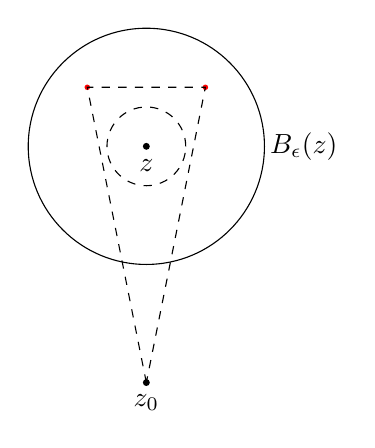
\begin{tikzpicture}
			\def \h{1.5}
			\def \hsmol{0.5}
			\def \del{0.25}
			\def \length{3}
			\def \theta{60} % in degrees
			\fill (0, 0) circle (1.25pt);
			\fill[red] (\h/2, \h/2) circle (1pt);
			\fill[red] (-\h/2, \h/2) circle (1pt);
			\draw[dashed] (0, -\length) -- (-\h/2, \h/2) -- (\h/2, \h/2) -- cycle;
			\node[] at (0, -\del) {$z$};
			\draw[] (0, 0) circle (\h);
			\draw[dashed] (0, 0) circle (\hsmol);
			\fill (0, -\length) circle (1.25pt);
			\node[] at (0, -\length-\del) {$z_0$};
			\node[] at (\h+2*\del, 0) {$B_\epsilon(z)$};
		\end{tikzpicture}
	\end{center}
	Let $z \in \Omega$ be arbitrary. We show that $F'(z) = f(z).$\\
	Since $\Omega$ is open, we can find $\epsilon > 0$ such that $B_\epsilon(z) \subset \Omega.$ We can choose points $z_1, z_2$ (in red) that belong to $B_\epsilon(x)$ such that $z$ in the interior of the triangle $T$ formed by $z_0, z_1, z_2$ (the dashed triangle).\\
	Note that $\widehat{T} \subset \Omega.$\\
	By \cref{lem:compcover}, there exists a (compact) $C \subset \Omega$ such that $\widehat{T} \subset \operatorname{int} C.$\\
	Let $\delta > 0$ be such that $B_\delta(z) \subset \operatorname{int} T.$ (The dashed circle is $B_\delta(z)$.)\\
	Now for all $h \neq 0$ such that $z + h \in B_\delta(z),$ we can use \nameref{prop:stronkgours} to conclude that
	\begin{align*} 
		F(z + h) - F(z) &= \int_{z_0}^{z+h} f(\xi) \mathrm{d}\xi - \int_{z_0}^{z} f(\xi) \mathrm{d}\xi\\
		&= \int_{z}^{z+h} f(\xi) \mathrm{d}\xi.
	\end{align*}
	The remainder of the proof then proceeds identically as earlier.
\end{proof}


\cif*\label{thm:cif2}
\begin{flushright}\hyperref[thm:cif]{\upsym}\end{flushright}
\begin{proof}
	First, we show that
	\begin{equation*} 
		\int_{\gamma}^{} \dfrac{f(\xi)}{\xi - z} \mathrm{d}\xi = \int_{\gamma_\epsilon}^{} \dfrac{f(\xi)}{\xi - z} \mathrm{d}\xi,
	\end{equation*}
	where $\gamma_\epsilon(t) = z + \epsilon e^{it},\;t \in [0, 2\pi]$ for any $\epsilon > 0$ small enough that $\overline{B_\epsilon(z)} \subset B_r(p).$
	\begin{center}
		\begin{tikzpicture}[decoration={markings,% switch on markings
			mark=at position .5 with {\arrow[line width=1mm]{stealth};}}
			]
			\def \r{7.5}
			\def \eps{2.5}
			\def \dist{4}
			\def \del{0.45}
			\fill (\dist, 0) circle (1.25pt) node[below]{$z$};
			\fill (0, 0) circle (1.25pt) node[below]{$p$};
			
			\draw[postaction={decorate}] (\r,0) arc (0:180:\r);
			\node[] at (0, \r+\del) {$\gamma'$};
			\draw[postaction={decorate}] (-\r,0) arc (180:360:\r);
			\node[] at (0, -\r-\del) {$\gamma''$};
			
			\draw[postaction={decorate}] (\eps+\dist,0) arc (0:180:\eps);
			\node[] at (\dist, \eps+\del) {$\gamma_\epsilon'$};
			\draw[postaction={decorate}] (-\eps+	\dist,0) arc (180:360:\eps);
			\node[] at (\dist, -\eps-\del) {$\gamma_\epsilon''$};

			\draw[postaction={decorate}] (-\r, 0) -- (\dist-\eps, 0);
			\node[] at (-\r/2, -\del) {$L_1$};
			
			\draw[postaction={decorate}] (\dist+\eps, 0) -- (\r, 0);
			\node[] at ({(\dist + \eps + \r)/2}, {-\del}) {$L_2$};
		\end{tikzpicture}
	\end{center}
	As shown in the figure, we get two paths as follows:
	\begin{align*} 
		L' &= L_1 * (\overline{\gamma_\epsilon'}) * L_2 * \gamma',\\
		L'' &= \gamma'' * (\overline{L_2}) * (\overline{\gamma_\epsilon''}) * (\overline{L_1}).
	\end{align*}
	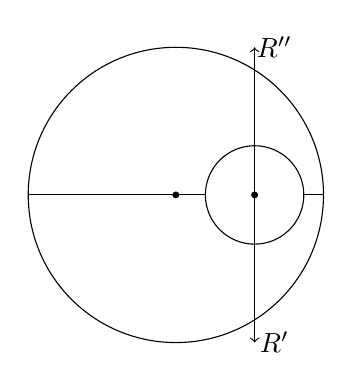
\begin{tikzpicture}[scale=0.25]
		\def \r{7.5}
		\def \eps{2.5}
		\def \dist{4}
		\def \del{1}
		\fill (\dist, 0) circle (5pt);
		\fill (0, 0) circle (5pt);
		\draw[] (\r,0) arc (0:180:\r);
		\draw[] (-\r,0) arc (180:360:\r);
		\draw[] (\eps+\dist,0) arc (0:180:\eps);
		\draw[] (-\eps+	\dist,0) arc (180:360:\eps);
		\draw[] (-\r, 0) -- (\dist-\eps, 0);
		\draw[] (\dist+\eps, 0) -- (\r, 0);
		\draw[->] (\dist,0) -- (\dist,\r);
		\node[] at (\dist + \del, \r) {$R''$};
		\draw[->] (\dist,0) -- (\dist,-\r);
		\node[] at (\dist + \del, -\r) {$R'$};
	\end{tikzpicture}
	Note that $L'$ is contained in the star-shaped region $(\mathbb{C}\setminus R')\cap \Omega$ and $L''$ in $(\mathbb{C}\setminus R'')\cap\Omega.$ In these star-shaped regions, the function $\xi \mapsto \dfrac{f(\xi)}{\xi - z}$ is holomorphic. \\
	Thus, by \nameref{cor:starprimitive}, we see that
	\begin{equation*} 
		\int_{L'}  \dfrac{f(\xi)}{\xi - z}\mathrm{d}\xi = \int_{L''} \dfrac{f(\xi)}{\xi - z}\mathrm{d}\xi = 0.
	\end{equation*}
	Adding the two integrals and using the facts $\gamma = \gamma'*\gamma'',$ $\gamma_\epsilon = \gamma_\epsilon' * \gamma_\epsilon'',$ we see that
	\begin{equation} \label{eq:gammaequality}
	 	\int_{\gamma}^{} \dfrac{f(\xi)}{\xi - z} \mathrm{d}\xi = \int_{\gamma_\epsilon}^{} \dfrac{f(\xi)}{\xi - z} \mathrm{d}\xi.
	\end{equation} 
	
	\hrulefill
	
	Now, we look at the integral on the right.
	\begin{align*} 
		\int_{\gamma_\epsilon}^{} \dfrac{f(\xi)}{\xi - z} \mathrm{d}\xi &= \int_{\gamma_\epsilon}^{} \dfrac{f(\xi) - f(z)}{\xi - z} \mathrm{d}\xi + \int_{\gamma_\epsilon}^{} \dfrac{f(z)}{\xi - z} \mathrm{d}\xi\\
		&= \int_{\gamma_\epsilon}^{} \dfrac{f(\xi) - f(z)}{\xi - z} \mathrm{d}\xi + f(z)\int_{\gamma_\epsilon}^{} \dfrac{1}{\xi - z} \mathrm{d}\xi\\
		&= \int_{\gamma_\epsilon}^{} \dfrac{f(\xi) - f(z)}{\xi - z} \mathrm{d}\xi + 2\pi if(z). & (*)
	\end{align*}
	We show that the integral in $(*)$ is zero.
	\begin{align*} 
		\left|\int_{\gamma_\epsilon}^{} \dfrac{f(\xi) - f(z)}{\xi - z} \mathrm{d}\xi\right| &\le \sup_{\xi\in B_\epsilon(z)}\dfrac{|f(\xi) - f(z)|}{|\xi - z|}(2\pi\epsilon)\\
		&=\sup_{\xi\in B_\epsilon(z)}\dfrac{|f(\xi) - f(z)|}{\epsilon}(2\pi\epsilon)\\
		&=2\pi \sup_{\xi\in B_\epsilon(z)}|f(\xi) - f(z)|.
	\end{align*}
	As we let $\epsilon \to 0,$ we see that the integral in $(*)$ goes to $0.$ Thus, letting $\epsilon \to 0$ in \cref{eq:gammaequality} yields the result.
\end{proof}



\holoanalytic*\label{cor:holoanalytic2}
\begin{flushright}\hyperref[cor:holoanalytic]{\upsym}\end{flushright}
\begin{proof}
	Fix $p \in \Omega.$ Since $\Omega$ is open, there exists some $r > 0$ such that $\overline{B_r(p)} \subset \Omega.$ Choose any such $r.$\\
	Let $z \in B_r(p).$ By \nameref{thm:cif}, we see that
	\begin{equation*} 
		f(z) = \dfrac{1}{2\pi i}\int_{\gamma}^{} \dfrac{f(\xi)}{\xi - z} \mathrm{d}\xi,
	\end{equation*}
	where $\gamma(t) = p + re^{it}$ for $t \in [0, 2\pi].$
	\begin{align*} 
		f(z) &= \dfrac{1}{2\pi i}\int_{\gamma}^{} \dfrac{f(\xi)}{\xi - z} \mathrm{d}\xi\\
		&=\dfrac{1}{2\pi i}\int_{\gamma}^{} \dfrac{f(\xi)}{\xi - p - (z - p)} \mathrm{d}\xi\\
		&= \dfrac{1}{2\pi i}\int_{\gamma}^{} \dfrac{f(\xi)}{(\xi - p)\left(1 - \frac{z - p}{\xi - p}\right)} \mathrm{d}\xi.
	\end{align*}
	Note that $z$ is fixed and $\xi$ varies over $\partial B_r(p)$ and thus, $|z - p| \lneqq |\xi - p| = r$ and hence,
	\begin{align*} 
		f(z) &= \dfrac{1}{2\pi i}\int_{\gamma}^{} f(\xi)\sum_{k=0}^{\infty}\dfrac{(z - p)^k}{(\xi - p)^{k+1}} \mathrm{d}\xi.
	\end{align*}
	Let $M > 0$ be such that $|f(\xi)| < M$ for all $\xi \in \partial B_r(p).$ (Which exists since $f$ is holomorphic and in particular, continuous.)\\
	Let $\rho \vcentcolon= \dfrac{|z - p|}{r}.$ Then, the sum $\sum f(\xi)\dfrac{(z - p)^k}{(\xi - p)^{k+1}}$ is dominated by $\sum (M/r)\rho^k$ and thus, by Weierstrass' M-test, the series converges uniformly. This lets us switch the sum and integral as
	\begin{align*} 
		f(z) &= \dfrac{1}{2\pi i}\sum_{k=0}^{\infty}\int_{\gamma}^{} f(\xi)\dfrac{(z - p)^k}{(\xi - p)^{k+1}} \mathrm{d}\xi\\
		&=\dfrac{1}{2\pi i}\sum_{k=0}^{\infty}(z - p)^k\left(\int_{\gamma}^{} \dfrac{f(\xi)}{(\xi - p)^{k+1}} \mathrm{d}\xi\right)\\
		&= \sum_{k=0}^{\infty}\left(\dfrac{1}{2\pi i}\int_{\gamma}^{} \dfrac{f(\xi)}{(\xi - p)^{k+1}} \mathrm{d}\xi\right)(z - p)^k.
	\end{align*}
	Note that $\dfrac{1}{2\pi i}\displaystyle\int_{\gamma}^{} \dfrac{f(\xi)}{(\xi - p)^{k+1}} \mathrm{d}\xi$ is independent of $z$ and thus, the above shows that $f$ admits a power series representation on $B_r(p).$
\end{proof}

\cauchest*\label{thm:cauchest2}
\begin{flushright}\hyperref[thm:cauchest]{\upsym}\end{flushright}
\begin{proof}
	Differentiate \cref{eq:holopowser} and put $z = p$ to get $a_k = \dfrac{1}{k!}f^{(k)}(p).$\\
	Comparing with \cref{eq:powsercoeff}, we get
	\begin{align*} 
		\left|f^{(k)}(p)\right| &= \dfrac{k!}{2\pi}\left|\int_{\gamma_R}^{} \dfrac{f(\xi)}{(\xi - p)^{k+1}} \mathrm{d}\xi\right|\\
		&\le \dfrac{k!}{2\pi}\sup_{\xi \in B_R(p)}|f(\xi)|\dfrac{1}{R^{k+1}}(2\pi R)\\
		&=\frac{k!}{R^k}\sup_{B_R(p)}|f|.
	\end{align*}
\end{proof}


\boundedentire*\label{thm:boundedentire2}
\begin{flushright}\hyperref[thm:boundedentire]{\upsym}\end{flushright}
\begin{proof}
	Let $f$ be entire and bounded. Let $M = \displaystyle\sup_\mathbb{C}|f|.$\\
	Fix $p = 0.$ The power series \cref{eq:holopowser} converges for all $z \in \mathbb{C}.$\\
	Fix $k \ge 1.$ By \nameref{thm:cauchest}, we see
	\begin{equation*} 
		|f^{(k)}(0)| \le \dfrac{k!M}{R^k}
	\end{equation*}
	for every $R > 0.$ Letting $R \to \infty,$ we see that $f^{(k)}(0) = 0.$\\
	As $k$ was arbitrary, we see that the power series simply reduces to $f(z) = a_0,$ as desired.
\end{proof}

\cauchyintegral*\label{thm:cauchyintegral2}
\begin{flushright}\hyperref[thm:cauchyintegral]{\upsym}\end{flushright}
\begin{proof}
	\begin{align*} 
		\int_{\gamma}^{} f(z) \mathrm{d}z &= \int_\gamma u\mathrm{d}x - v\mathrm{d}y + i\int_\gamma u\mathrm{d}y + v\mathrm{d}x\\
		&= \iint_{\operatorname{int}\gamma}(v_x + u_y)\mathrm{d}(x, y) + i\iint_{\operatorname{int}\gamma}(u_x - v_y)\mathrm{d}(x, y)\\
		&= 0.
	\end{align*}
	We have used the fact that the vector field $(u, v)$ is continuously differentiable and appealed to \nameref{thm:greens}. The last $0$ follows by virtue of the CR equations.
\end{proof}


\constnbd*\label{lem:constnbd2}
\begin{flushright}\hyperref[lem:constnbd]{\upsym}\end{flushright}
\begin{proof}
	Note that an open and connected set in $\mathbb{C}$ is path connected.\\
	Let $c = f(p).$\\
	We know that $f\equiv c$ in a neighbourhood $B_\delta(p).$ Choose any $q \in \Omega$ distinct from $p.$ We show that $f(z) = c$ for all $z$ in a neighbourhood of $q$ and thus, complete the proof.\\
	Choose any continuous path $\gamma:[0, 1] \to \Omega$ such that $\gamma(0) = p$ and $\gamma(1) = q.$\\
	Define $S \subset [0, 1]$ as
	\begin{equation*} 
		S \vcentcolon= \{t \in [0, 1] \mid f \equiv c\text{ in a neighbourhood of }\gamma(t)\}.
	\end{equation*}
	We know that $S$ is nonempty since $0 \in S.$ Moreover, $[0, \zeta] \subset S$ for some $\zeta > 0.$ (Consider the intersection of $\gamma([0, 1])$ with $B_\delta(p).$)\\
	Set
	\begin{equation*} 
		m \vcentcolon= \sup\{t_0 \in [0, 1] \mid [0, t_0] \subset S\} > 0.
	\end{equation*}
	We shall show that $m = 1$ and that will complete the proof.\\
	Let $d \vcentcolon= \operatorname{dist}\Big(\gamma\big([0, 1]\big), \partial \Omega\Big).$\\
	Note that $d > 0$ since $\gamma\big([0, 1]\big)$ is compact and does not intersect $\partial\Omega.$\\
	Select $\eta > 0$ such that 
	\begin{equation*} 
		\left|s - t\right| < \eta \implies \left|\gamma(s) - \gamma(t)\right| < \frac{d}{3}.
	\end{equation*}
	(Note that $\gamma$ is continuous and thus, uniformly continuous.)

	The important thing to remember is that for each $z_0 \in \Omega,$ the power series representation of $f$ is valid throughout $B_r(z_0)$ where $r = \operatorname{dist}(z_0, \partial \Omega).$

	Choose $t_0 \in S$ such that $m - \frac{\eta}{2} < t_0 \le m$ such $[0, t_0] \subset S.$ (Exists by definition of $m.$)\\
	Thus, $f \equiv c$ in a neighbourhood of $\gamma(t_0).$\\
	Thus, the power series of $f$ at $\gamma(t_0)$ reduces to the constant and thus, $f \equiv c$ on $B_d(\gamma(t_0)).$ (Recall $d$ defined earlier.)

	Also, note that $|t_0 - m| < \eta/2 < \eta$ and thus, $\left|\gamma(t_0) - \gamma(m)\right| \le \dfrac{d}{3},$ by choice of $\eta$ and thus, $\gamma(m) \in B_d(\gamma(t_0)).$\\
	Thus, $f\equiv c$ in a neighbourhood of $m.$

	In fact, given any $t \in \left(m - \dfrac{\eta}{2},  m + \dfrac{\eta}{2}\right) \cap [0, 1],$ $f \equiv c$ in a neighbourhood of $t.$ (Since any such $t$ would be at distance at most $\eta$ from $t_0$.)

	Thus, if $m < 1,$ then we would get a contradiction as we would get an $m' > m$ which is in the set $\{t_0 \in [0, 1] \mid [0, t_0] \subset S\}.$

	This shows that $m = 1.$
\end{proof}


\preiden*\label{thm:preiden2}
\begin{flushright}\hyperref[thm:preiden]{\upsym}\end{flushright}
\begin{proof}
	(i) $\implies$ (ii) is trivial.

	(ii) $\implies$ (iii).\\
	Let $(p_n)$ and $p$ be as above. By continuity of $f,$ we get that $f(p) = 0.$ That is, $f^{(0)}(p) = 0.$\\
	Assume that (iii) is not true. We arrive at a contradiction.\\
	By our assumption, there exists $k \in \mathbb{N}$ such that $f^{(k)}(p) \neq 0.$ Choose the smallest such $k.$ Then, the power series around $p$ reads
	\begin{equation*} 
		f(z) = (z - p)^k(a_k + a_{k+1}(z - p) + \cdots).
	\end{equation*}
	Note that $a_k \neq 0.$\\
	Let $g(z) \vcentcolon= a_k + a_{k+1}(z - p) + \cdots.$ That is, $f(z) = (z - p)^kg(z)$ with $g$ continuous at $p.$\\
	Since $g(p) = a_k \neq 0,$ there exists a neighbourhood $U$ of $p$ such that $g(z) \neq 0$ for any $z \in U.$\\
	Choose $N$ sufficiently large such that $p_N \in U$ and $p_N \neq p.$ Then, note that $g(p_N) \neq 0$ and $(p_N - p)^k \neq 0.$ However, $g(p_N)(p_N - p)^k = f(p_N) = 0.$ A contradiction.

	(iii) $\implies$ (i).\\
	If $f^{(k)}(p) = 0$ for all $k \ge 0,$ then $f \equiv 0$ on a neighbourhood of $p.$ The result then follows by the previous lemma.
\end{proof}


\morera*\label{thm:morera2}
\begin{flushright}\hyperref[thm:morera]{\upsym}\end{flushright}
\begin{proof}
	Since holomorphy is a local property, it is enough to prove that $f$ is holomorphic on each disc $D \subset \Omega.$ WLOG, we may assume that $\Omega$ is a disc. (In particular, $\Omega$ will be convex.)

	We first construct a primitive for $f.$ Fix $z_0 \in \Omega.$ Define $F:\Omega \to \mathbb{C}$ as
	\begin{equation*} 
		F(z) \vcentcolon= \int_{z_0}^{z} f(\xi) \mathrm{d}\xi.
	\end{equation*}
	Let $h \neq 0$ be small enough that $z + h \in \Omega.$ Then,
	\begin{align*} 
		F(z+h) - F(z) &= \int_{z_0}^{z+h} f(\xi) \mathrm{d}\xi - \int_{z_0}^{z} f(\xi) \mathrm{d}\xi\\
		&= \int_{z_0}^{z+h} f(\xi) \mathrm{d}\xi + \int_{z}^{z_0} f(\xi) \mathrm{d}\xi\\
		&= \int_T f + \int_{z}^{z+h} f(\xi) \mathrm{d}\xi\\
		&= \int_{z}^{z+h} f(\xi) \mathrm{d}\xi,
	\end{align*}
	where $T$ is the triangle with vertices $z_0, z, z+h.$

	The remainder of the proof now goes identically as that of \cref{cor:primexists}. (See proof \hyperref[cor:primexists2]{here}.)

	Thus, we get that $F' = f.$ Since $F$ is holomorphic, it is infinitely differentiable and so is $f.$
\end{proof}


\montel*\label{cor:montel2}
\begin{flushright}\hyperref[cor:montel]{\upsym}\end{flushright}
\begin{proof}
	To show that $f$ is holomorphic, it is sufficient to prove it in the case that $\Omega$ is a disc.\\
	Note that $f$ is continuous since the convergence is uniform. We show that $\displaystyle\int_T f = 0$ for any triangle $T \subset \Omega.$ The holomorphy of $f$ will then follow from \nameref{thm:morera}.

	Let $T \subset \Omega$ be an arbitrary triangle. Note that $T$ is compact and thus, $f_n \to f$ on $T.$ This gives us that
	\begin{align*} 
		\int_T f = \int_T\left(\lim_{n\to \infty}f_n\right) = \lim_{n\to \infty}\int_T f_n = 0,
	\end{align*}
	as desired.
	
	\hrulefill
	
	Now, we show that $f_n' \to f'$ uniformly on compact sets.\\
	Let $K \subset \Omega$ be compact.\\
	Set $d \vcentcolon= \operatorname{dist}(K, \partial\Omega).$ (If $d = \infty,$ then set $d \vcentcolon= 43.$)

	Let $z \in K.$ Then, $\overline{B_{d/3}(z)} \subset \overline{B_{2d/3}(z)} \subset \Omega.$ Applying \nameref{thm:cauchest} ($k = 1$) gives us:
	\begin{align*} 
		|f_n'(z) - f'(z)| &\le \left(\dfrac{d}{3}\right)^{-1}\sup_{\xi \in B_{d/3}(z)}\left|f_n(\xi) - f(\xi)\right|.
	\end{align*}
	Let $\tilde K = \displaystyle\bigcup_{z \in K}B_{2d/3}(z).$ Then, $\overline{\tilde K} \subset \Omega$ is compact. Moreover, we have
	\begin{equation*} 
		\bigcup_{z \in K}B_{d/3}(z) \subset \overline{\tilde{K}}.
	\end{equation*} 
	Thus, the above inequality gives us:
	\begin{align*} 
		|f_n'(z) - f'(z)| &\le \left(\dfrac{d}{3}\right)^{-1}\sup_{\xi \in \overline{\tilde K}}\left|f_n(\xi) - f(\xi)\right|.
	\end{align*}
	Note that the RHS $\to 0$ as $n \to 0$ since $(f_n)$ uniformly converges to $f.$ Moreover, the inequality is true for all $z \in K$ and thus, we see that $f_n \to f'$ uniformly on $K.$
	
	\hrulefill
	
	More elaboration on the last part:\\
	Let $\epsilon > 0$ be given, then there exists $N \in \mathbb{N}$ such that $\left|f_n(\xi) - f(\xi)\right| < \epsilon$ for all $n \ge N$ and all $\xi \in \overline{\tilde K}.$ (This is because of uniform convergence of $f_n$ on $\overline{\tilde K}.$)

	Choose any such $N.$ Then, we have 
	\begin{equation*} 
		\sup_{\xi \in \overline{\tilde K}}\left|f_n(\xi) - f(\xi)\right| \le \epsilon
	\end{equation*}
	for all $n \ge N.$ In turn, we have, for all $z \in K,$
	\begin{equation*} 
		|f_n'(z) - f'(z)| \le 3\epsilon/d
	\end{equation*}
	for all $n \ge N.$ This proves the desired uniform convergence.
\end{proof}



\constmodconst*\label{lem:constmodconst2}
\begin{flushright}\hyperref[lem:constmodconst]{\upsym}\end{flushright}
\begin{proof}
	Writing $f = u + iv$ as usual, we see that 
	\begin{equation*} 
		u^2 + v^2 \equiv c.
	\end{equation*}
	If $c = 0,$ then we are done. Assume $c \neq 0.$\\
	Differentiating the above w.r.t. $x$ gives us
	\begin{equation*} 
		uu_x + vv_x = 0. \quad (*)
	\end{equation*}
	Similarly, differentiating w.r.t. $y$ gives us
	\begin{equation*} 
		uu_y + vv_y = 0.
	\end{equation*}
	Using CR equations, the last equation can be re-written as
	\begin{equation*} 
		-uv_x + vu_x = 0. \quad (**)
	\end{equation*}
	$(*)$ and $(**)$ together give us
	\begin{equation*} 
		\begin{bmatrix}
			u & v\\
			v & -u
		\end{bmatrix}
		\begin{bmatrix}
			u_x\\
			v_x
		\end{bmatrix}
		= \begin{bmatrix}
			0\\
			0
		\end{bmatrix}.
	\end{equation*}
	Note that $\det\begin{bmatrix}
			u & v\\
			v & -u
		\end{bmatrix} = c \neq 0$ and thus, $u_x = v_x \equiv 0$ on $\Omega.$\\
	This gives us that $f' \equiv 0$ on $\Omega$ and thus, $f$ is constant, since $\Omega$ is connected.
\end{proof}


\maxmod*\label{thm:maxmod2}
\begin{flushright}\hyperref[thm:maxmod]{\upsym}\end{flushright}
\begin{proof}
	Let $p$ be as in the theorem. Let $D$ be an open disc containing $p$ such that $\left|f(p)\right| \ge \left|f(z)\right|$ for all $z \in D.$\\
	Let $r > 0$ be arbitrary such that $\overline{B_r(p)} \subset D.$ Let $\gamma(t) \vcentcolon= p + re^{it}$ for $t \in [0, 2\pi].$ Then, \nameref{thm:cifreal} gives us
	\begin{align*} 
		f(p) &= \dfrac{1}{2\pi i}\int_{\gamma}^{} \dfrac{f(z)}{z - p} \mathrm{d}z\\
		&= \dfrac{1}{2\pi}\int_{0}^{2\pi} f(p + re^{it}) \mathrm{d}t.
	\end{align*}
	Hence,
	\begin{align*} 
		\left|f(p)\right| &\le \dfrac{1}{2\pi}\int_{0}^{2\pi} \left|{f(p + re^{it})}\right| \mathrm{d}t\\
		&\le \dfrac{1}{2\pi}\int_{0}^{2\pi} \left|{f(p)}\right| \mathrm{d}t\\
		&= \left|f(p)\right|.
	\end{align*}
	Thus,
	\begin{equation*} 
		\left|f(p)\right| = \dfrac{1}{2\pi}\int_{0}^{2\pi} \left|{f(p + re^{it})}\right| \mathrm{d}t
	\end{equation*}
	or
	\begin{equation*} 
		\int_{0}^{2\pi} \left[\left|f(p)\right| - \left|{f(p + re^{it})}\right|\right] \mathrm{d}t = 0.
	\end{equation*}
	Note that the integrand is nonnegative and continuous. Thus, the integrand must be identically zero. This gives us that
	\begin{equation*} 
		\left|f(p)\right| = \left|f(p + re^{it})\right|
	\end{equation*}
	for all $t \in [0, 2\pi]$ and all $r$ sufficiently small.

	Thus, $|f|$ is constant in a neighbourhood of $p.$ By \cref{lem:constmodconst}, we see that $f$ is constant in a neighbourhood of $p.$ Since $\Omega$ is connected, we appeal to \cref{lem:constnbd} and conclude that $f$ is constant on $\Omega.$
\end{proof}


\openmapping*\label{thm:openmapping2}
\begin{flushright}\hyperref[thm:openmapping]{\upsym}\end{flushright}
\begin{proof}
	Let $U$ be an arbitrary open subset of $\Omega.$\\
	Let $w_0 \in f(U)$ be arbitrary. We show that $f(U)$ contains a neighbourhood of $w_0.$ This will prove the theorem.\\~\\
	Let $z_0 \in U$ be such that $f(z_0) = w_0.$ Let $\epsilon > 0$ be such that $V \vcentcolon= B_\epsilon(z_0) \subset U$ and $f(z) \neq w_0$ for $|z - z_0| = \epsilon.$ (Such a choice of $\epsilon$ is possible because the zeroes of $z\mapsto f(z) - w_0$ are isolated.)\\~\\
	It follows that $0 < \delta \vcentcolon= \inf\{\left|f(z)\right| \mid |z - z_0| = \epsilon\}.$ (Since the $\inf$ is actually attained on a compact set.)\\
	\begin{blockquote}
	\textbf{Claim.} $B_{\delta/2}(w) \subset f(V).$
	\begin{proof} 
		Let $w \in \mathbb{C}$ be such that $\left|w - w_0\right| < \delta/2.$ For the sake of contradiction, assume that $w \notin f(V).$ \\
		By assumption, the function $g:V\to\mathbb{C}$ given by $z\mapsto f(z) - w$ does not vanish.\\
		Since $g$ is non-vanishing and holomorphic, so is $1/g.$

		By \cref{cor:modinterior}, it follows that
		\begin{align*} 
			\dfrac{1}{\left|g(z_0)\right|} &< \sup\left\{\dfrac{1}{\left|f(z) - w\right|} \;\Big|\; z \in \partial V \right\}. \quad (*)
		\end{align*}
		We estimate the quantity on the right side as follows:\\
		For $z \in \partial V,$ we know that $\left|f(z) - w_0\right| \ge \delta.$ We then see that
		\begin{align*} 
			\left|f(z) - w_0\right| &\ge \delta\\
			\implies \left|f(z) - w_0\right| - \left|w_0 - w\right| &> \dfrac{\delta}{2} > 0\\
			\implies \left|f(z) - w_0\right| - \left|w_0 - w\right| &= \left|\left|f(z) - w_0\right| - \left|w_0 - w\right|\right|.
		\end{align*}
		Using reverse triangle inequality, we see that
		\begin{align*} 
			\left|f(z) - w\right| &\ge \left|f(z) - w_0\right| - \left|w_0 - w\right|\\
			&\ge \delta - |w_0 - w|\\
			\implies \dfrac{1}{\left|f(z) - w\right|} &\le \dfrac{1}{\delta - |w_0 - w|}\\
			\implies \sup_{z \in \partial V}\dfrac{1}{\left|f(z) - w\right|} &\le \dfrac{1}{\delta - |w_0 - w|}.
		\end{align*}
		We now return to $(*)$ with the above inequality and the fact that $\left|w - w_0\right| = |g(z_0)|$ to obtain
		\begin{equation*} 
			\dfrac{1}{\left|w - w_0\right|} \le \dfrac{1}{\delta - \left|w - w_0\right|}.
		\end{equation*}
		The above gives us $\left|w - w_0\right| \ge \dfrac{\delta}{2},$ a contradiction.
	\end{proof}
	\end{blockquote}
	The above claim proves the desired result.
\end{proof}